\documentclass[msc,lith,english]{liuthesis}

%%%%%%%%%%%%%%%%%%%%%%%%%%%%%%%%%%%%%%%%%%%%%%%%%
% Imports
%%%%%%%%%%%%%%%%%%%%%%%%%%%%%%%%%%%%%%%%%%%%%%%%%
%\usepackage[english]{babel}
\usepackage[utf8]{inputenc}
\usepackage[backend=biber,sorting=none,hyperref]{biblatex}
\usepackage{mathtools}
\usepackage{dsfont}
\usepackage{tikz}
\usetikzlibrary{topaths,calc}
\usepackage{algorithm2e}

%%%%%%%%%%%%%%%%%%%%%%%%%%%%%%%%%%%%%%%%%%%%%%%%%
% Settings
%%%%%%%%%%%%%%%%%%%%%%%%%%%%%%%%%%%%%%%%%%%%%%%%%
\department{Institutionen för datavetenskap}
\departmentenglish{Department of Computer and Information Science}
\departmentshort{IDA}

\supervisor{Peter Jonson}
\examiner{???}
\titleenglish{A Faster Algoritm for Solving the No-Rainbow Problem}
\subtitleenglish{100\% rainbow-free guarantee}
\titleswedish{En snabbare algoritm för No Rainbow problemet}
\thesissubject{Datavetenskap}

\publicationyear{2023}
\currentyearthesisnumber{001}
\dateofpublication{2023-01-20}

\addbibresource{thesis.bib}

\author{Edvard Thörnros}

\begin{document}

%%%%%%%%%%%%%%%%%%%%%%%%%%%%%%%%%%%%%%%%%%%%%%%%%
% Intro
%%%%%%%%%%%%%%%%%%%%%%%%%%%%%%%%%%%%%%%%%%%%%%%%%
\chapter{Introduction}
\label{chaIntro}
The faster something can be done, the faster technology can iterate.
A part of this is finding faster algorithms for known hard problems.
One such hard problem is the no rainbow problem, which is NP-complete.
The no rainbow problems asks if there is a surjective node coloring of an $r$-regular hypergraph.

Rephrased, the no rainbow problem asks if we can assign each node a color.
In a graph with $r$ nodes per edge -- each edge connects $r$ different nodes.
All $r$ colors should be represented in the entire graph.
No edge should connect all $r$ colors.
A node coloring that satisfies these constraints is a solution to the no rainbow problem.

An edge that connects all $r$ colors is called a rainbow edge -- hence the name of the problem.
The no rainbow problem is a variant of the constraint satisfaction problem.
\cite{sourceNoRainbow}

\section{Motivation}
The no rainbow problem is related to the phylogenetic decisiveness problem. The
phylogenetic decisiveness problem asks if a potential ancestral tree for a
species of animals could possibly be correct, given only parts of the
information about the ancestry of a species. \cite{sourcePhylogeneticDecisiveness} \cite{sourceNoRainbow}

Problems are always worth studying. Understanding a problem and presenting a
solution can in itself give insights and understanding into harder problems. 
A well-made algorithm can be used as a building block to solve even harder problems.

% Honestly, this is grasping at straws.
The no rainbow problem is a studied NP-hard problem and could give some insight into the P versus NP problem.
The P versus NP problem is one of the millennium problems -- a solution would have enormous ramifications for our lives.

% TODO: Read https://ieeexplore.ieee.org/document/9616390
% TODO: https://www.researchgate.net/publication/350673538_Exact_Algorithms_for_No-Rainbow_Coloring_and_Phylogenetic_Decisiveness

\section{Research questions}
\begin{enumerate}
  \item Is there a faster* deterministic algorithm that solves the no rainbow problem than the one suggested by Ghazaleh Parvini and David Fernandez-Baca \cite{sourceNoRainbow}?
  \item Is there a faster* randomized algorithm that solves the no rainbow problem than the one suggested by Ghazaleh Parvini and David Fernandez-Baca \cite{sourceNoRainbow}?
  % \item How can a solution to the no rainbow problem be found, understood, modeled and presented?
  % \item What insights into algorithms are found by studying the no rainbow problem?
  \item How fast* is the fastest* possible algorithm for solving the no rainbow problem? 
\end{enumerate}
*Speed is defined by asymptotic computational complexity.

\section{Aim}
The aim of this study is to find an asymptotically faster algorithm that solves
the no rainbow problem. Then present the algorithm and its proof in an accessible way.

\section{Delimitations}
This study will focus on the theoretical no rainbow problem.
Implementing the algorithms is not part of this study.

%%%%%%%%%%%%%%%%%%%%%%%%%%%%%%%%%%%%%%%%%%%%%%%%%
% Background
%%%%%%%%%%%%%%%%%%%%%%%%%%%%%%%%%%%%%%%%%%%%%%%%%
\chapter{Background}
\label{chaBackground}
The no rainbow problem is quite complex and can be understood in a lot of different ways.
To understand the problem as broadly as possible a few different areas of discrete mathematics are needed.

\section{Equivalence classes and equivalence relations}
Equivalence classes are used to group things that are equal in some sense.
This requires we have a set of objects and an binary operator we can use to check if they are equal.
In this general case we use $\sim$ as the operator.

$$
  a \sim b \implies \textit{$a$ is related to $b$ under the equivalence relation ($\sim$)}
$$

A common way of defining equivalence relations is to map the objects to their image and then use equality.
More generally we can define it using:
$$
  a \sim b \iff f(a) = f(b)
$$
Where $f(a)$ is the image of $a$.

For example:
$$
  a \sim b \iff (a \bmod 3) = (b \bmod 3) : \quad a, b \in \mathds{Z}
$$

Here we send each object to their image -- that is their remained after division by 3 -- and then compare them.
Here we get 3 equivalence classes $\{[0], [1], [2]\}$. All integers are mapped into exactly one of these 3 equivalence class.

The representative of a class is the element that has itself as image. In other words, $f(a) = a \iff a$ is a representative.
\cite[Section 7.3]{sourceArmen} \cite[Section 1.2]{sourceAATA}

\section{Graphs}
Graphs consist of a set of edges and a set of nodes.
Nodes are usually presented as circles with edges connecting the circles as lines, as presented in \ref{figGraphExample}.
Usually an edge is some kind of relationship. 
A graph is a very powerful and general tool for modeling many problems.

\begin{center}
\begin{figure}[h]
\centering
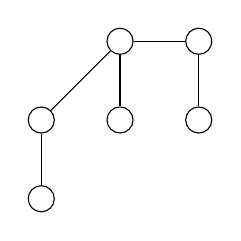
\begin{tikzpicture}[main/.style = {draw, circle}]
    \node[main] (A) {};
    \node[main] (B) [left of=A] {};
    \node[main] (C) [below of=A] {};
    \node[main] (D) [left of=C] {};
    \node[main] (E) [left of=D] {};
    \node[main] (F) [below of=E] {};

    \draw (A) -- (B);
    \draw (A) -- (C);
    \draw (B) -- (D);
    \draw (B) -- (E);
    \draw (F) -- (E);
\end{tikzpicture}
  \caption{An example of a graph.}
  \label{figGraphExample}
\end{figure}
\end{center}

\cite[Chapter 1]{sourceDiestel}
\cite[Chapter 1]{sourceGWA}
\cite[Section 9.1]{sourceArmen}

% Does this add anything?

\section{Hyper Graphs}
A hyper graph is similar to a normal graph.
But in a hyper graph edges connect multiple nodes, usually more than 2.
A hyper edge that is 2-regular is a "normal" graph.
The "normal" graph can be seen as a special case of the hyper graph.

Another way of phrasing it is that an edge is a set of nodes instead of a pair.

A hyper graph is the kind of graph the no rainbow problem is interesting for.

\begin{center}
\begin{figure}[h]
\centering
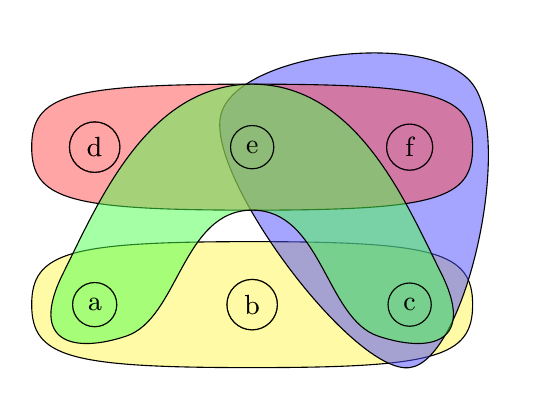
\begin{tikzpicture}[main/.style = {draw, circle}]
    \node[main] (a) at (0,2) {a};
    \node[main] (b) at (2,2) {b};
    \node[main] (c) at (4,2) {c};
    \node[main] (d) at (0,4) {d};
    \node[main] (e) at (2,4) {e};
    \node[main] (f) at (4,4) {f};

    \begin{scope}[fill opacity=0.5]
    \filldraw[fill=yellow!70] 
        plot [smooth cycle, tension=1.5]
        coordinates {
          ($(a)+(-0.8,0)$) 
          ($(b)+(0,0.8)$) 
          ($(c)+(0.8,0)$)
          ($(b)+(0,-0.8)$) 
        };

    \filldraw[fill=blue!70] 
        plot [smooth cycle, tension=0.8]
        coordinates {
          ($(c)+(0,-0.8)$) 
          ($(f)+(0.8,0.8)$) 
          ($(e)+(-0.4,0.4)$)
        };

    \filldraw[fill=red!70] 
        plot [smooth cycle, tension=1.5]
        coordinates {
          ($(d)+(-0.8,0)$) 
          ($(e)+(0,0.8)$) 
          ($(f)+(0.8,0)$)
          ($(e)+(0,-0.8)$) 
        };

    \filldraw[fill=green!70] 
        plot [smooth cycle, tension=1.0]
        coordinates {
          ($(c)+(-0.4,-0.4)$) 
          ($(c)+(0.4,0.4)$) 
          ($(e)+(0,0.8)$)
          ($(a)+(-0.4,0.4)$) 
          ($(a)+(0.4,-0.4)$) 
          ($(e)+(0,-0.8)$)
        };

    \end{scope};

    \node[main] (a) at (0,2) {a};
    \node[main] (b) at (2,2) {b};
    \node[main] (c) at (4,2) {c};
    \node[main] (d) at (0,4) {d};
    \node[main] (e) at (2,4) {e};
    \node[main] (f) at (4,4) {f};
\end{tikzpicture}
  \caption{An example of a hyper graph.}
  \label{figHyperGraphExample}
\end{figure}
\end{center}

% Show the other way of rendering them

The hyper graph shown in figure \ref{figHyperGraphExample} is $3$-regular.
A hyper graph is $r$-regular if and only if all edges connect $r$-different nodes.
\cite{sourceHyper}

\subsection{Node coloring as related by the no rainbow problem}
A node coloring is a mapping from nodes to colors.
There are usually constraints on what colors can be part of an edge.
The color of a node is denoted as $c(a)$, where $a$ is the node and $c$ is the coloring.
Since a coloring is a mapping it can be thought of as a function that takes you from a node to the color of the node.
A color is usually a letter or a number.

The constraints added in the no rainbow problem are
\begin{enumerate}
  \item No edge can have all r-colors -- no rainbow edges
  \item All colors have to be represented in the graph -- the coloring is surjective
\end{enumerate}

An example of a valid coloring in the no rainbow problem for the graph presented above is $c(d)=0, c(b)=1, c(*)=2$, where $*$ denotes all other nodes.
There are a lot more valid colorings, though this coloring is particularly simple.
The validity of a coloring is dictated by the edges added in the graph.
A hyper-graph with the maximum number of edges (called a complete graph) has no valid no-rainbow coloring.
A hyper-graph without any edges is trivial to find a no-rainbow coloring for.
The cases in between are the main topic of this thesis.

\cite{sourceHyper}
% Is a complete r-regular subgraph enough to disprove there is a no-rainbow coloring? Yes.

\section{Asymptotic Computational Complexity}
Sometimes called asymptotic time complexity is a theoretical basis for evaluating algorithms.
The asymptotic computational complexity of an algorithm shows how the run time
of the implemented algorithm scales given infinitely large inputs.

There are multiple kinds of asymptotic computational complexity. The most used
one -- and the one presented in this paper -- is the "big-O" notation. "Big-O"
gives the highest upper bound of this theoretical runtime -- or the worst-case
computational complexity. Examples usually make things clearer, so let us look at an algorithm.
One intuition for the computational complexity is to "count the number of steps".

\begin{algorithm}
\caption{A slow exponentiation algorithm}\label{algDivSlow}
\KwData{$a,b \in \mathds{Z}, \quad b \le 0$}
\KwResult{$a^b$}
\DontPrintSemicolon
\SetKwFunction{FExp}{Exp}
\SetKwProg{Fn}{Function}{:}{end}

\Fn{\FExp{$a$, $b$}}{
  $x \gets 1$ (Runs 1 time.)\;
  \While(\lparen Runs $b$ times, with $K$ steps.\rparen){$b \le 0$}{
    $x \gets x * a$\; 
    $b \gets b - 1$\;
  }
  \KwRet $x$ (Runs 1 time.)\;
}
\end{algorithm}

We assume multiplication can be done in constant time -- it always takes at most $K$ units of time to do a multiplication.
The algorithm \ref{algDivSlow} will perform $ 2 + Kb $ steps, where $K$ is some
constant. We can rewrite this using "Big-O" notation as $O(1 + Kb)$. The expression can be
simplified to remove constants that become insignificant if the
input is sufficiently large. Then we get $O(2 + Kb) = O(b)$, since both $1$ and $K$ are constants. 
Normally the asymptotic time complexity is defined based on the size of the input not the magnitude of the value.
The size of the input is measured in number of bits called $n$. When we add a bit to $b$ we multiply the steps by 2,
thus $O(b) = O(2^n)$.

There are other ways to reason to this conclusion.
One other way is to realize we have to visit all numbers between $0$ and $b$.
In binary this means visiting all possible combinations of 0s and 1s that are needed to describe $b$.
We have 2 choices for $n$ bits. All combinations have to be visited. So we visit $O(2^n)$ numbers in the worst case.
\cite[Chapter 3]{sourceAlgoBook}

A common error is to claim algorithm \ref{algDivSlow} runs in $O(n)$ -- linear time. This is incorrect.

Aside from $O$ there is also $O*$. $O*(x^n)$ allows us to discard polynomial factors as well. For example $O*(x^n)$ would allow the algorithm to run in $O(2^nx^n)$.

\section{Computational Classes}

\chapter{Related Work}
Exhaustively studies of the no rainbow problem have not been done. There are however a plethora of related problems.
These related problems are more broadly studied.

\section{Exact Algorithms for No-Rainbow Coloring and Phylogenetic Decisiveness}
"Exact Algorithms for No-Rainbow Coloring and Phylogenetic Decisiveness" are currently the fastest algorithms.
Two algorithms are presented. One deterministic and one non-deterministic. Both
algorithms use the idea of searching similar potential solutions for a fixed
depth, and then trying again. The non-deterministic algorithm samples the
solution space randomly, while the deterministic algorithm samples a specific
structure. \cite{sourceNoRainbow}

\begin{center}
\begin{figure}[h]
\centering
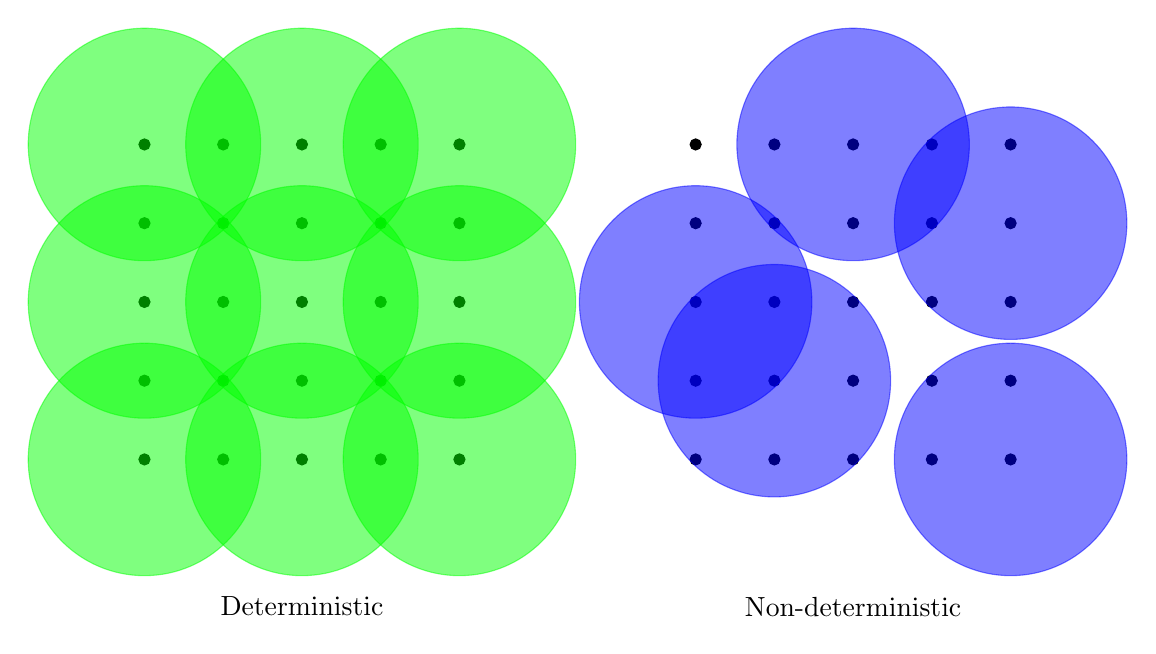
\begin{tikzpicture}
  \newcommand\circleRadius{42pt}

  \foreach \x in {0,...,4}{
    \foreach \y in {0,...,4}{
      \filldraw[black] (\x,\y) circle (2pt);
    }
  }

  \foreach \x in {0,2,4}{
    \foreach \y in {0,2,4}{
      \filldraw[green, opacity=0.5] (\x,\y) circle (\circleRadius);
    }
  }
  \draw (2,-1.5) node[label=below:Deterministic]{};

  % SHIFTED +(4+3,0)
  \foreach \x in {7,...,11}{
    \foreach \y in {0,...,4}{
      \filldraw[black] (\x,\y) circle (2pt);
    }
  }

  \filldraw[blue, opacity=0.5] (8,1) circle (\circleRadius);
  \filldraw[blue, opacity=0.5] (7,2) circle (\circleRadius);
  \filldraw[blue, opacity=0.5] (11,0) circle (\circleRadius);
  \filldraw[blue, opacity=0.5] (9,4) circle (\circleRadius);
  \filldraw[blue, opacity=0.5] (11,3) circle (\circleRadius);
  \draw (9,-1.5) node[label=below:Non-deterministic]{};


\end{tikzpicture}
  \caption{A visualization of how the deterministic and non-deterministic algorithms tries different colorings. Each black dot is a potential solution. The colored circles show the searched adjacent solutions.}
  \label{figHyperGraphExample}
\end{figure}
\end{center}

\printbibliography

\appendix
\chapter{Changes after feedback seminar (2022-11-25)}
Removed 2 research questions. Added motivation. Added aim. Added delimitations. Fixed typos of multi graph and hyper graph. Corrected typo in title. Moved background to its own chapter. Took feedback from Don and replaced "which" with "that".

\end{document}
